\documentclass{article}

\usepackage[ngerman]{babel} % german translation for document elements
\usepackage{hyperref}       % clickable links
\usepackage{amsmath}        % formeln
\usepackage{amssymb}        % mathe symbole

% for figures and subfigures
\usepackage{graphicx}
\usepackage{caption}
\usepackage{subcaption}

% ////////////////////////////////////////////////

\usepackage{xcolor}
\definecolor{mred}{HTML}{fe163d}
\definecolor{mgreen}{HTML}{009052}
\DeclareRobustCommand{\@todo(viktor):}[1]{\textcolor{mred}{@todo:} \textcolor{mred}{#1}} 
\DeclareRobustCommand{\at}[1]{\textcolor{mgreen}{#1}}
% % override the writing commands to be empty
\DeclareRobustCommand{\@todo(viktor):}[1]{} 
\DeclareRobustCommand{\at}[1]{}


% ////////////////////////////////////////////////

\title{Wave Function Collapse auf Graphen}
\author{Viktor Berengar Askan Graf von Westarp}

\begin{document}

\maketitle
\pagebreak

\tableofcontents
\pagebreak

\section{Einleitung}
\subsection{Motivation}
\subsection{Problemstellung und Ziel}
\subsection{Problemlösung}
\subsection{Aufbau der Arbeit}

\section{Hintergrund}

    \subsection{Model Synthesis}
        \at{@citation model synthesis}
        Mit dem \textit{Model Synthesis} Algorithmus können, basiert auf einem 3D Beispielmodell, eine große Menge an ähnlichen 3D Modellen prozedural generiert werden. Das synthesierte/generierte Model wird auf einem 3D Gitter iterativ generiert, indem jedem Knotenpunkt des Gitters ein Teil des Beispielmodells zugewiesen wird. Das Beispiel muss vorher in kleinere gleichgroße Bauteile zerlegt werden. Jedem Knotenpunkt wird zu Beginn die Menge aller Bauteile als seine Auswahlmöglichkeiten zugewiesen. Mit jeder Iteration wird bei einem Knotenpunkt ein Bauteil seiner Zustandsmenge ausgewählt. Danach werden alle Nachbarn geprüft, so dass sie nur noch passende Bauteile in ihrer Zustandsmenge behalten. Hierfür wird eine globale Suche verwendet, andere Methoden beschränkten sich zuvor nur auf lokale Suchen. Eine globale Suche ist besser, weil jedes Bauteil einen weitreichenden Einfluss auf das gesamte Gitter haben kann.

        \at{@incomplete Consistency}
        Damit die Ausgabe eine sinnvolle Anordnung der Bauteile ergibt, werden nur Bauteile die nebeneinander in einer bestimmten Richtung im Beispiel sind, in der Ausgabe nebeneinander in dieser Richtung platziert. Dadurch ist garantiert, dass jede kleine Region der Ausgabe mindestens einer Region im Beispiel gleicht. Da an jedem Knotenpunkt meist mehr als ein Bauteil passen würde und die Auswahl per Zufall geschieht, ist es unwahrscheinlich, dass die Ausgabe genau dem Beispiel im ganzen gleicht. Bei der Auswahl des Bauteils für einen Knoten wird die Wahrscheinlichkeit jedes Bauteils auch mit seiner Häufigkeit im Beispiel gewichtet, wodurch über eine große Menge an Ausgaben die Häufigkeit einzelner Bauteile der tatsächlichen Häufigkeit im Beispiel gleicht. Für eine einzelne Ausgabe bedeutet dies, dass die globale Verteilung der Bauteile auch tendenziell der Verteilung im Beispiel gleicht. 
        \at{@incomplete Resemblance}
        \at{@visual from ms paper}

        Die selbe Methodik kann auch auf 2D Gittern angewendet werden; dies wird dann \textit{Texture Synthesis} genannt. Desweiteren kann der Algorithmus um andere Techniken der prozeduralen Generierung erweitert werden, so können z.B. andere beliebige Beschränkungen auf die Ausgabe angewendet werden. \at{@visual}
        \at{@incomplete NP-Completeness}
        \at{@incomplete Unused: Soft Constraints \& Symmetry \& iterative small area solves}

    \subsection{Wave Function Collapse}
        \at{@citation wfc}
        \textit{Wave Function Collapse} ist eine Weiterentwicklung des Model Sythesis Algorithmus. Die Kernidee der Generierung mittels einem Beispiel bleibt und wird um drei Aspekte erweitert. Anstatt nur Bauteile nebeneinander anzuordnen, können nun auch überlappende Teile des Beispiels automatisch aus einem Beispiel extrahiert werden. In jeder Iteration wird die Zelle mit der niedrigsten Entropie zuerst betrachtet. Bei Bauteil-basierten Beispielen werden Symmetrien von Bauteilen zur kompakteren Definition ausgenutzt.
        \at{@incomplete renamings: model synthesis/wfc, observe \& collapse, vertex/cell, widerspruch}

        \at{@incomplete generalization to NxN Überlappung}


        Die Reihenfolge in der die Zellen observiert werden, hat einen Einfluss auf die Laufzeit. Bei Model Synthesis werden Zellen einfach nach ihrer Reihenfolge im Gitter abgearbeitet. Der Vorteil ist, dass keine Suche der nächsten Zelle nötig ist, aber es hat zum Nachteil, dass die Ausgabe sichtbare Artefakte enthällt. Man kann erkennen, ob zuerst die Reihen oder erst die Spalten abgearbeitet wurden \at{@visual von github links}. Wäre bekannt welche Zelle den meisten Fortschritt zur Lösung und die geringste Chance auf einen Widerspruch birgt, könnte stets diese Zelle zuerst betrachtet werden (\at{@incomplete} NP-Hardness). 

        Einfacher ist es eine Heuristik zu definieren, die simpel zu berechnen ist und meistens einen besseren Ansatz bietet. Hierfür wird die Entropie als Maß eingeführt. Sie beschreibt das Maß an Ungewissheit über den finalen Zustand einer Zelle. Ist eine Zelle observiert, hat sie nur noch einen Zustand und die Entropie ist minimal, während eine Zelle mit vielen Möglichkeiten eine hohe Entropie hat. Die Entropie gibt auch Information darüber wie sehr eine Zelle durch ihre Umgebung beschränkt wird. Sie mit der Formel der Shannon-Entropie \at{@citation} berechnet.


        Der Zerteilung eines Beispiels in Bauteile muss manuell passieren. Soll nun ein Bauteil auch in einer anderen Orientierung oder Spiegelung in der Ausgabe vorkommen müssen diese Variationen explizit angelegt werden. Will man nun ein Bauteil leicht verändern, so muss man auch alle Variationen manuel anpassen. Um diesen aufwendigen Prozess zu automatisieren definiert Gumin eine Gruppe von Symmetriearten mit denen eine Nutzerin ihre Bauteile annotieren kann. Der Algorithmus erkennt diese Annotationen und generiert vor Beginn automatisch die Variationen.
        \at{@incomplete interesting but unused for this work}
        % @todo(viktor): \ref{fig:wfc_gumin}

\subsection{Gitter, Graphen, Triangulierung, Voronoi}

\section{Konzept}
    \subsection{Einschränkung des Algorithmus und Idee zur Erweiterung}
    \subsection{Wave Function Collapse auf Graphen}
        \subsubsection{Output Graphen}

    \subsection{Regelextrahierung \at{@naming}}
        \at{@citation merrel}
        \at{@flow Die Absätze sind okay aber ihre Reihenfolge muss überdacht werden}
        
        Ziel des Wave Function Collapse ist es, eine große Anzahl lokal ähnlicher Ausgaben zu generieren. Ähnlichkeit wird erreicht, wenn jede kleine Region der Ausgabe zu Regionen der Eingabe passt. Der Algorithmus weist jeder Zelle des Output-Graphen einen Zustand zu, so dass zwei Bedingungen gelten. Erstens muss der Zustand einer Zelle in mindestens einer Richtung mit den Zuständen aller Nachbarzellen überlappen können. Zweistens soll die Richtung der Überlappung möglichst ähnlich der Richtung zum Nachbarn sein.
        
        Ein Umfeld ist die Region um einen Pixel der Eingabe. Ein Zustand besteht aus dessen Umfeld und Frequenz in der Eingabe. In der Eingabe, die ein Quadratgitter ist, können Umfelder in acht Richtungen überlappen; im Norden, Süden, Westen, Osten und in den diagonalen Himmelsrichtungen. 
        
        Die Regeln welche Zustände überlappen und welche nicht, werden vor Beginn des Collapse aus der Eingabe extrahiert. Dafür wird für jeden Pixel der Eingabe sein Umfeld notiert. Liegt ein Pixel am Rand der Eingabe, so kann es sein, dass sein Umfeld zum Teil außerhalb der Eingabe liegne würde. Ist die Eingabe so erstellt, dass der linke Rand an den rechten Rand passt, bzw. der Obere an den Unteren, so nimmt man für das Umfeld von Randpixeln auch die Pixel vom der anderen Seite hinzu. Ist dies nicht erwünscht für eine Eingabe so können diese Umfelder einfach verworfen werden. Dies wird in dieser Arbeit als Wrapping bezeichnet, wobei Wrapping für die vertikalen Ränder und die horizontalen Ränder separat erlaubt oder verboten werden kann.
        Jedes einzigartige Umfeld wird ein möglicher Zustand der einer Zelle zugewiesen werden kann. Tritt ein Umfeld mehr als einmal in der Eingabe auf, so wird dem entsprechenden Zustand eine höhere Frequenz zugewiesen. Aus der Gesamtanzahl an Zuständen und deren Frequenzen lässt sich die Wahrscheinlichkeit jedes Zustands berechen. Dies wird im Collapse genutzt, damit nicht nur lokale Ähnlichkeit sondern auch die globale Verteilung von Umfeldern der Eingabe ungefähr ähnelt (\at{@incomplete} das nicht nur hier so knapp sagen sondern auch später nochmal erwähnen). 
        
        % @todo(viktor): \ref{fig:extract_wrapping}
        
        \at{@placement Das ist eher Implementierung}
        Während des Collapse werden die Regeln, welche Zustände überlappen, nach jedem Schritt für alle benachbarten Zellen geprüft. Da sich diese Eigenschaft aber nicht während des Verlauf des Algorithmus ändert, kann eine Datenstruktur zuvor zur Speicherung erstellt werden. Die Überlappungs-Lookuptabelle gibt für jedes Zustandspaar die Richtungen an, in denen die Zustände überlappen. Wenn Zellen nun geprüft werden, kann nun aus der Lookuptabelle abgelesen werden, wodurch viel wiederholte Arbeit vermieden wird.
        
        Ist der Output-Graph ein Quadratgitter können die diagonalen Richtungen bei der Betrachtung entfallen, ohne dass es einen Einfluss auf die Qualität der Ausgabe hat. Die reguläre Struktur führt dazu, dass wenn für eine Zelle A der Nachbar von A im Norden(An) passt und der Nachbar im Westen von An passt, dann muss auch der Nachbar von A im Nordwesten passen. \at{@wording}
        
        \at{@incomplete Symmetrie und Transitivität der Regeln}
        
        Ein Umfeld wird im Umfang dieser Arbeit als ein 3x3 Gitter von Pixeln definiert. Es können auch andere Formen und Größen gewählt werden, aber diese müssen zu den genutzen Eingaben passen, damit die in den Eingaben existierenden Muster optimal genutzt werden. Wird das Umfeld zu klein gewählt, können nur Ausschnitte der gewünschten Muster erhalten werden, die Muster selbst gehen verloren. Während ein zu großes Umfeld auch die Anordnung der Muster in der Eingabe erhällt, was unerwünscht ist und im extremen Fall dazu führt, dass nur noch exakte Kopien der Eingabe ohne Variation in der Ausgabe vorkommen.
        
        Den Zellen des Output-Graphen sind, nach einem erfolreichem Collapse, je ein Zustand zugewiesen. Dieser kann aber nicht direkt durch sein Umfeld dargestellt werden, da das Umfeld eines Zustands zur Ermittlung der Überlappungen dient und deswegen aus mehr als einem Pixel, also einem Farbwert besteht. In dieser Arbeit wird der Pixel in der Mitte des Umfelds als der tatsächliche Farbwert einer Zelle zur Darstellung genutzt.
    
\section{Umsetzung}
    \subsection{Generierung von Voronoi-Graphen}
    
    \subsection{Collapse Cells - Step \at{@naming}}
    
    \subsection{Überlappung und Heat \at{@naming}}
    
    \at{ @flow}
    In einem 2D Gitter sind die Nachbarn jeder Zelle per Definition des Gitters in festen Richtungen und Abständen zu finden. Bei Graphen ist diese Anordnung frei. 
    Die Überlappung von zwei Zuständen hängt von der Richtung zwischen den beiden Umfeldern, also von der Verschiebung des einen Umfeld zum anderen. 
    Während der Propagate-Phase werden die möglichen Zustände von Nachbarzellen auf Überlappung geprüft.
    Ein Zustand einer Zelle ist möglich\at{@translation}, wenn er mit mindestens einem Zustand jeder Nachbarzelle überlappen kann.
    Die Überlappung zweier Zustände hängt von der Richtung zwischen den Umfeldern der Zustände abhängt ab. Das heißt, dass für den Nachbar im Norden einer Zelle nur die Überlappung der Zustände im Norden relevant ist. Die Richtung zu einer Nachbarzelle auf einem Graphen wird als der Vektor von Mittelpunkt der Zelle zum Mittelpunkt der Nachbarzelle definiert. Der wichtigste Unterschied ist, dass die Richtung nun nicht mehr auf die acht Himmelsrichtungen (N, NO, O, SO, S, SW, W, NW) beschränkt ist. 
    
    \@todo(viktor):{ beliebige Richtungen müssen auf die acht Himmelsrichtungen gemappt werden}
    \\ \@todo(viktor):{ wir können nur die 8 HR aus der Eingabe extrahieren, interpolation(bilineares sampling) nicht möglich da wir diskrete zustände haben}
    \\ \at{@visual Vergleich von Hexgrid mit Heat 1 und Heat 2}
    
    
    
    \subsection{Backtracking}
    
    
    
\section{Ergebnisse und Diskussion}

\section{Fazit}
\subsection{Vergleich zum Original}
\subsection{Mögliche Anwendungsbereiche?}
\subsection{Ausblick und zukünftige Forschung}

\section{Literaturverzeichnis}
% figure out how to use maybe this: \bibliography{}


% ////////////////////////////////////////////////
\pagebreak

\section{Hintergrund}
    \at{@incomplete Einleitender Satz, was zu prozeduraler Generierung}

\subsection{Gitter, Graphen, Triangulierung, Voronoi}
    \at{@incomplete Definition von Gitter und Graph in dieser Arbeit}
    
    \subsubsection{Oskar Stålberg}
        \at{@incomplete WFC on irregular quadrilations, Oskar Stålberg}
        \begin{itemize}
        \item usage in Bad North and Town Scaper
        \item aperiodic infinite deterministic irregular relaxed quadrilateral grids
        \end{itemize}

        
\section{Konzept}
    \@todo(viktor):{alles nachfolgende lesen und duplikate weiter nach vorne holen oder auslassen}
    \at{@incomplete Heuristik für Heat oder manuell?}
    \at{@incomplete Welche Nachbarn hat eine Zelle? Wie beeinflusst eine Zelle seine Nachbarn im Graph und was hat Heat damit zutun? Zustand/Richtungsmengen erklären.}

    \subsection{Einschränkung des Algorithmus und Idee zur Erweiterung}
        
        Die ursprüngliche Form des Wave Function Collapse nimmt in 2D Pixelmuster oder Tilesets als Eingabe und produziert darauß wieder 2D Muster. 
        Pixel liegen stets auf einem quadratischen Gitter. Bei Tilesets ist die grafische Gestaltung des Tiles uneingeschränkt. Dennoch sind die Tiles selbst quadratisch. Dies schränkt die Gestaltung des Inhalts der Tiles in sofern ein, dass die Kanten zu anderen Kanten passen müssen. Auch bei 3D Inputs werden die Modelle in blockförmige Bausteine zerschnitten, damit der Collapse auf einem 3D Gitter von Würfeln arbeiten kann.

        Man beschränkt sich auf regelmäßige quadratische Gitter, da ihre Struktur bestimmte Vorteile mit sich bringt. Benachbarung von Zellen ist implizit durch die Struktur des Gitters mitgeliefert. Eine Zelle des Ausgabegitters ist durch seine Koordinaten im Gitter definiert und seine Nachbarn lassen sich einfach durch Schritte in vier festen Richtungen in 2D oder sechs Richtungen in 3D finden. Diese Eigenschaft gilt durch die Regelmäßigkeit des Gitters für alle Zellen gleichermaßen. Dies ist nützlich, da die Benachbarungsregeln, die aus der Eingabe herausgezogen werden, eben auch auf einem regelmäßigem Gitter basieren und direkt im Algorithmus verwendet werden können.

        Der Nachteil dadurch, dass die Generierung immer auf einem regelmäßigem quadratischen Gitter läuft, ist, dass die Ausgabe im Ganzen Artefakte des Gitter aufweist. Vertikale und horizontale Linien können im Pixelgitter dargestellt werden, aber bei diagonalen oder frei geformte Kurven und Linien müsste eine Zelle des Ausgabegitters anteilmäßig ausgefüllt sein, was aber nicht möglich ist. Eine Zelle kann immer nur einen diskreten finalen Zustand wählen. Es kommt zu Aliasing.

        Wenn man sich den Kern des Wave Function Collapse Algorithmus genauer anguckt, erkennt man, dass die Entscheidung, welchen Zustand eine Zelle erhällt, nur von den möglichen Zuständen ihrer Nachbarn abhängt. Deren Zuständ geschränken die Menge aller in der Eingabe existierenden Zustände, auf genau diese, die in der Eingabe nebeneinander gefunden wurden. Dabei ist auf dem Gitter immer eindeutig, dass z.B. die Zelle N nördlich einer betrachteten Zelle M, nur Zustände wählen kann die in der Eingabe nördlich von einem von M's Zuständen gefunden wurde. Damit der Algorithmus die Menge an möglichen Zuständen einer Zelle finden kann, braucht es also nur eine Funktion die aus der tatsächlichen Richtung von M zu N die betrachtete Richtung der Benachbarungregeln ergibt. Im Gitter ist gibt diese Funktion meißt die Identität; die Richtung zum Nachbarn ist die Richtung für die Regeln. 

        Wenn man mit WFC eine Ausgabe erstellen will, die sich selbst tiled \at{@translation} (also linker Rand gleich rechter Rand und so) kann man eine imaginäre Kante von einer Zelle am rechten Rand zu einer Zelle am linken Rand erstellen und dem Algorithmus definieren dass diese Benachbarung in Richtung Osten geht. Nun sind die Ränder des Gitters benachbart und das Ergebnis ist, dass die Ränder, wenn eine Lösung gefunden wird, zueinander passen. Wenn man dies für einen Rand macht, so ist die Form der Zellen mit ihren Nachbarn nicht mehr eine flache Ebene, sondern die Oberfläche eines Zylinders(ohne Deckel und Boden). Verbindet man auf die selbe Weise auch den anderen Rand, ist die Form nun ein Torus. Der Algorithmus selbst muss also nur auf diese Weise angepasst werden, um auf anderen Anordnungen von Zellen zu funktionieren.

    \at{@incomplete Diagonale Regeln, besseres Sampling der Eingabe, Regelmengen, höhere Entropie durch Strictness}

    \subsection{Wave Function Collapse auf Graphen}

        \subsubsection{Output Graphen}

        Wave Function Collapse arbeitet normalerweise mit einem regelmäßigem Gitter. Hier ist die Anordnung der Zellen eindeutig; die Position einer Zelle und welche Nachbarn sie hat und in welcher Richtung die relativ zur Zelle sind implizit in der Datenstruktur eingebaut. Bei einem Graphen müssen diese Informationen explizit gespeichert werden. Jede Zelle kann eine beliebige Position haben und beliebig viele Nachbar in beliebigen Richtungen haben. 

        Jede Kante des Graphen stellt eine Beschränkung des Lösungsraums dar. Bei einem Gitter ist jede Zelle, mit Ausnahme der Zellen am Rand, gleichermaßen beschränkt, jedoch kann die Anordnung des Graphen dazu führen dass einzelne Zelle weniger und andere stärker eingeschränkt werden. Eine Zelle mit zehn Nachbarn muss in einen Zustand collapsen welcher zu den Zuständen der zehn Nachbaren passt.

        Ein Graph kann somit stark beschränkte und schwach beschränkte Regionen enthalten, während dass Gitter uniforme Beschränkung auf Zellen ergibt. Zur Erinnerung: es muss nur eine Zelle eine Widerspruch verursachen damit der Algorithmus fehlschlägt. Also sind solche Regionen starker Beschränkung besonderns entscheident für die Chance einen validen Output zu generieren, weil hier der Lösungsraum am kleinsten ist.

        \at{@incomplete Entropy erwähnen und für Regionen mit einer Grafik von der App darstellen}

    
\section{Umsetzung}

\subsection{Generierung von Voronoi-Graphen}
    \@todo(viktor):{ Erklärung der Generierung separat zur erklärung der Anforderung an den Graphen auf dem der Algorithmus laufen soll \\}
    \begin{itemize}
        \item Der Algorithmus arbeitet auf einem gegebenen Graphen. Die Verteilung der Zellen kann regelmäßig oder ohne Struktur sein. Es muss kann auch über den Graphen hinweg variieren. Jede Zelle hat eine 2D Position und jeder Zelle müssen alle ihre Nachbarzellen zugewiesen werden. Zellen sind benachbart, wenn sie eine Kante teilen. Eine Kante sind alle Punkte die gleichweit von zwei Zellenmittelpunkten entfernt sind. 
        \item In meiner Anwendung erstelle ich die Graphen prozedural aus einfachen Mustern oder mittels Zufallsprinzip. 
        \item Meine generierten Graphen sind immer planar, da ich immer dem selben Ablauf folge. Erst erstelle ich eine Menge an 2D Punkten, die wie gesagt eine beliebige Anordnung habe. Dann erstelle ich auf diesen Punkten eine Delaunay-Triangulierung. Das Gegenstück einer solchen Triangulierung ist ein Voronoi-Diagramm. Man findet es in dem man die Eckpunkte der Dreiecke als Mittelpunkte der Voronoizellen nimmt und die Kanten der Dreiecke enden in den Nachbarzellen jeder Zelle. Da Zellen am Rand von diesem Voronoi-Diagramm nach außen unendlich groß sind, begrenzen wir diese Zellen auf eine freigewählte rechteckige Fläche. 
        \item Zu Beginn des Wave Function Collapse werden alle Zellen mit einer Superposition aller möglichen Zustände initialisiert.
    \end{itemize}

    \at{@incomplete Warum generieren wir die Graphen und kurz wie und welche Settings gibt einem die App dafür. }
    \at{@visual Beispiele der Generierung}

    \at{@placement}
    Man kann ein regelmäßiges Quadratgitter als eine spezielle Form von Voronoigraph ansehen. Jedes Quadrat kann als eine Voronoizelle angesehen werden, welche genau alle Punkte die am nächsten zu seinem Mittelpunkt enthällt. Die Nachbarn können nun explizit über die Kanten der Voronoizelle gefunden werden. Zuvor waren diese auch implizit durch die Koordinate des Quadrats im Gitter gegeben.

    Für den Algorithmus ist diese Unterscheidung egal und er generiert die gleiche Art von Ausgaben ohne weitere Anpassungen. \at{@visual}
    Also können wir auch andere Voronoigraphen als Outputgraphen verwenden.

    Um einen Voronoigraphen zu generieren nutze ich die Eigenschaft, dass der duale Graph zu jedem Voronoigraph eine Delaunay-Triangulierung ist. Eine Delaunay Triangulierung kann man auf unterschiedlich Weise aus einer beliebigen Point-Cloud, einer Menge an Punkten im 2D Raum, generieren. Dies ist optimal für mich, da ich nun einfach eine Point-Cloud auf beliebige Weise, also mit oder ohne Struktur und so komplex oder simpel wie ich es will, erstellen und aus dieser ein validen Voronoigraph erhalten kann.

    \at{@incomplete Eigenschaften einer Delaunay-Triangulierung nennen}

    Für die Triangulierung habe ich mich ohne tiefere Beweggründe für den Boywer-Watson Algorithmus entschieden. Der Algorithmus generiert die Triangulierung iterativ in dem jeder Punkt nacheinander eingefügt wird und der Graph angepasst wird, so dass es wieder eine Delaunay-Triangulierung ist.
    Zur Hilfe erstellen wir ein Superdreieck, welches alle Punkte enthällt. Nun fügen wir einen Punkt ein und prüfen all bisher gefundenen Dreiecke, ob ihr Umkreis diesen Punkt enhällt. Ist der Punkt innerhalb des Umkreises kann das Dreieck nicht zur finalen Triangulierung gehören. Für alle diese Dreieck sammeln wir nun die Kanten. Jede Kante die nur einmal vorkommt ist teil der Hülle dieser Dreiecke, alle anderen Kanten sind innerhalb dieser Hülle, da sich zwei Dreiecke diese teilen. Diese inneren Kanten werden entfernt und für jede Ecke entlang der Hülle wird eine neue Kante zum eingefügten Punkt erstellt.
    Am Ende entfernt alle Kanten zur den Eckpunkten des Superdreiecks aus der Triangulierung und erhällt die Delaunay-Triagulierung der Point-Cloud.

    Aus der Triangulierung erstellen wir das Voronoidiagram indem wir die Eckpunkte als Mittelpunkte der Voronoizellen nehmen. Die Kanten sagen uns welche Zellen benachbart sind. Um die Kanten der Voronoizelle zu finden nehmen wir von alle Dreiecke in denen der Punkt liegt den Mittelpunkt des Umkreises. Die Umkreismittelpunkte sind die Ecken der Voronoizelle. Die Kanten finden wir indem wir die Punkte nach ihrem Winkel um den Mittelpunkt der Zelle sortieren und dann der Reihe nach verbinden.
    \at{@visual}

    Es ist normal, dass ein solches Voronoidiagram an den Rändern der Point-Cloud auch Zellen ergeben kann die auf einer Seite offen sind, weil die Kanten zwischen den Ecken der Zelle, den Umkreismittelpunkten, keinen Schnittpunkt haben. Ich habe mich dazu entschieden, bei solchen Zellen weitere Eckpunkte einzufügen, so dass das alle Zellen durch einen freigewählten rechteckigem Bereich begrenzt sind. Dafür prüfe ich ob ein Eckpunkt außerhalb des Bereichs liegt und finde dann den Schnittpunkt von der Kante zu dem Eckpunkt mit dem Rechteck des Bereichs und ersetze den Eckpunkt mit diesem Schnittpunkt. Dieser Schritt passiert so lange bis alle Eckpunkte innerhalb oder auf dem Rand des Bereichs liegen.
            Siehe Abbildung \ref{fig:voronoi_clipping}.

\subsection{Überlappung und Heat}
    % strictness to heat for now, support to overlap
    
\subsection{Collapse Cells - Step \at{@naming}}
    Der Algorithmus generiert die Ausgabe iterativ. Eine Iteration, ein Schritt, kann in vier Phasen geteilt werden: Search, Pick, Observe und Propagate.
    
    Zu Beginn wird die Zelle mit der geringsten Entropie gesucht, die noch nicht collapsed ist. Die Entropie einer Zelle wird als die Shannon-Entropy \at{@citation} der noch möglichen Zustände berechnet. 
    
    Es ist möglich, dass mehrere Zellen die gleiche Entropie haben. Zum Beispiel haben am Anfang, bevor dem ersten Schritt, sind alle Zellen in der Superposition aller Zustände, wodurch alle Zellen die selbe Entropie haben. Aus der Menge an gefundenen Zellen wird in diesem Fall in der Pick-Phase eine Zelle zufällig ausgewählt.

    In der Observe-Phase wird ein Zustand zufällig aus der Superposition ausgewählt und die Zelle collapsed. Die Wahrscheinlichkeit eines Zustands gewählt zu werden hängt von dessen Häufigkeit in der Eingabe ab. Dadurch generiert der Algorithmus Ausgaben die lokal ähnlich sind, sondern auch global eine ähnliche Verteilung an allen Mustern aufweisen.
            Die anderen Zustände werden entfernt was Einfluss auf die Nachbarzellen haben kann. 
    
    Danach beginnt die Propagate-Phase. Eine Liste aller geänderten Zellen wird mit der observierten Zelle initialisiert. Für jede Zelle in dieser Liste werden alle Nachbarn überprüft, ob nun einer der Zustände nicht mehr möglich ist. Solange mindestens ein Zustand der aktuellen Zelle zu einem Zustand der Nachbarzelle passt, also sie entsprechend der Richtung zum Nachbarn überlappen, dann behält die Nachbarzellen diesen Zustand. Ansonsten ist der Zustand nicht mehr möglich und wird entfernt. Sollte nun auch der letzte mögliche Zustand entfernt werden, so wurde ein Widerspruch erreicht. Der Graph kann nun nicht mehr gelöst werden. Sind nach der Prüfung aber noch Zustände möglich so, wird die Zelle der Liste zu prüfender Zelle angefügt.
    Diese Phase dauert so lange, bis sich keine Zellen mehr ändern.
    
\subsection{Backtracking}
    Wenn der Algorithmus einen Widerspruch entdeckt, muss nicht immer alle Arbeit verworfen werden. Gerade bei größeren oder komplizierteren Mustern oder Graphen ist es wahrscheinlich, dass beim ersten Versuch keine Lösung gefunden wird, weil die Komplexität den Lösungsraum stärker einschränkt. Wenn ein Widerspruch in einer Zelle aber nun nur von den direkten Nachbar abhängt, so ist es wahrscheinlich dass weiter entfernte bereits gelöste Zellen dennoch kompatibel sind. Um einen lokalen Widerspruch aufzulösen muss meistens nur lokal eine andere Entscheidung getroffen werden.

    Um Backtracking umzusetzen müssen mehr Informationen behalten werden als nur der Zustand des Gitters zum aktuellen Zeitpunkt. Will man nun wieder einen Schritt zurückgehen muss man wissen, welche Entscheidung man zuvor bereits getroffen hat um dessen Effekt rückgängig zu machen. Dabei genügt es nicht nur die Collapste Zelle und den Zustand wieder zu entfernen, weil jede Zelle von mehreren Nachbarn beeinflusst wird. Die Zustandsmenge einer Zelle ist die Schnittmenge der möglichen Nachbarzuständen der Nachbar. Somit kann es sein, dass ein Zustand A aus der Menge wegen mehreren Einschränkungen von mehreren Nachbarn fehlt. Nimmt man nun durch Backtracking eine dieser Einschränkungen wieder zurück, so ist es nicht offensichtlich, ob Zustand A nun wieder möglich ist, ohne alle Einschränkungen auf die Zelle neu zu berechnen.
    Entweder man macht die Änderung nur lokal rückgängig und berechnet immer alle Zellen neu, bis sich keine mehr ändern. Oder man speichert ab, zu welchem Zeitpunkt ein Zustand unmöglich geworden ist und prüft ob dieser Zeitpunkt nach dem Schritt zurück weiterhin in der Vergangenheit oder nun in der Zukunft liegt. Bei zweiterem müssen alle solche Zustände als wieder möglich betrachtet werden.
    Diese Art die Menge an Zuständen darzustellen ist gut, weil sich für jede Zelle die Zustandsmenge in jedem Schritt des Algorithmus immer nur verkleinert oder gleichbleibt. Ist ein Zustand durch die Nachbar unmöglich so wird er auch nie wieder an späterem Zeitpunkt möglich.

    Desweiteren wollen wir bereits gemachte Entscheidungen nicht noch einmal wiederholen, wenn diese zu einem Widerspruch führen werden. Die Entscheidungspunkte in der  Pick- und Observe-Phase können gleich behandelt werden. Wir können die List an Auswahlmöglichkeiten für später speichern und die ausgewählte Zelle oder den ausgewählten Zustand von der Liste entfernen. Kommen wir nun zu diesem Schritt zurück können wir einfach die nächste Möglichkeit auswählen und den Algorithmus normal weiterlaufen lassen.

    \@todo(viktor):{ Pseudo-Code oder Diagramme für Algorithmus and Backtracking?}

    In der Umsetzung speichere ich für jede Zelle eine Liste aller Zustände. Jeder Zustand ist entweder möglich und wurde noch nicht entfernt oder ist unmöglich und speichert den Zeitpunkt an dem er unmöglich wurde. Hierbei ist der Zeitpunkt einfach die Anzahl an Schritten des Algorithmus. 
    Für jeden Schritt des Algorithmus speichern wir nun die Liste der gefundenen Zellen in Search. Wenn in Pick eine Zelle ausgewählt wird, entfernen wir diese aus der Liste und wählen beim Backtracken nun eine andere. Ebenso speichern wir vor der Observe-Phase alle wählbaren Zustände und entfernen mit jedem Lösungsversuch den gewählten Zustand. 

    Nun haben wir unwissentlich auch eine Schwachstelle in den Algorithmus eingeführt. Wenn wir zuvor in der Search-Phase keine Zellen in Superposition mehr gefunden haben, waren alle Zellen tatsächlich collapsed. Nun kann es auch sein, dass alle Zellen, die wir finden, zu einem Widerspruch führen. Auch in der Observe-Phase war es unmöglich keinen Zustand mehr auswählen zu können, da eine Zelle mit leerer Zustandmenge bereits zuvor als Widerspruch identifiziert wurden wäre. 
    Um diese Fälle ordentlich zu behandeln können wir nun aber einfach auch in solchen Fällen einen Widerspruch deklarieren und Backtracken. Schließlich haben wir alle noch möglichen Entscheidungen bereits getroffen und ausgewertet und keine Lösung gefunden. Somit führt dieser Schritt zwar nicht direkt zu einem Widerspruch in einer Zelle, aber alle folgen Schritte werden irgendwann zu einem Widerspruch führen. Zu Bemerken ist, dass wenn auf diese Weise bis zum ersten Schritt gebacktrackt wird und auch die erste Entscheidung einen Widerspruch verursacht, so kann die Kombination aus Eingabe und Graph keine Ausgabe ergeben.

\pagebreak

\section{Notizen}
\begin{enumerate}
    \item Passive Form: In dieser Arbeit, im Umfang dieser Arbeit, diese Arbeit...
    \item Die Todos aufräumen und nur die fertigen Teile an Schlechtweg schicken
    \item die Ergebnisse festhalten
    \item planare Graphen raus
    \item mehr Grafiken - was besseres für das layout der beschriftungen finden
    \item Tippfehler und Korrekturlesen
\end{enumerate}

\subsection{Must do}
\begin{enumerate}
    \item prozedurale generierung
    \item wfc algorithmus erklären
    \item quadrat, regelmäßige und unregelmäßige gitter
    \item 8 statt 4 Directions in Extrahierung
    \item overlap / direction mask
    \item Heat und Heuristik zur verbesserung, erweiterungsmöglichkeiten mit simulated annealing und heating und cooling chance with heat
\end{enumerate}

\subsection{Can do}
\begin{enumerate}
    \item model synthesis
    \item Delaunay-Triangulierung
    \item Voronoi Diagramme
    \item Townscapers Gitter
    \item Vergleiche zwischen Algorithmen und Daten
    \item Ähnlichkeit zum Input
    \item wahrscheinliche Lösbarkeit und NP-Hardness
\end{enumerate}
% ////////////////////////////////////////////////

% @todo(viktor): should these be in order of usage?
\begin{figure}[ht]
    \centering
    \begin{minipage}{\linewidth}
        \rule{\linewidth}{0.4pt}
        
        \begin{enumerate}
        \item Read the input bitmap and count NxN patterns.
        \subitem (optional) Augment pattern data with rotations and reflections.
        \item Create an array with the dimensions of the output (called ''wave'' in the source). Each element of this array represents a state of an NxN region in the output. A state of an NxN region is a superposition of NxN patterns of the input with boolean coefficients (so a state of a pixel in the output is a superposition of input colors with real coefficients). False coefficient means that the corresponding pattern is forbidden, true coefficient means that the corresponding pattern is not yet forbidden.
        \item Initialize the wave in the completely unobserved state, i.e. with all the boolean coefficients being true.
        \item Repeat the following steps: \begin{enumerate}
            \item Observation: \begin{enumerate}
                \item Find a wave element with the minimal nonzero entropy. If there is no such elements (if all elements have zero or undefined entropy) then break the cycle (4) and go to step (5).
                \item Collapse this element into a definite state according to its coefficients and the distribution of NxN patterns in the input.
            \end{enumerate}
            \item Propagation: propagate information gained on the previous observation step.
        \end{enumerate}
        \item By now all the wave elements are either in a completely observed state (all the coefficients except one being zero) or in the contradictory state (all the coefficients being zero). In the first case return the output. In the second case finish the work without returning anything.
        \end{enumerate}
        
        \rule{\linewidth}{0.4pt}
    \end{minipage}
    
    \caption{Wave Function Collapse Algorithmus nach Gumin \cite{gumin}}
    
    \label{fig:wfc_gumin}
\end{figure}
\begin{algorithm}
    \caption{Generierung eines Graphen}
    \label{alg:graph_gen}
        
    \begin{enumerate}
    \item Erstelle eine Menge an Punkten
    
    \item Generiere die Delaunay-Triangulierung der Punkte
    \subitem Die Ecken und Kanten aller Dreiecke bilden den Graphen
        
    \item Erstelle die Voronoi-Zellen aus der Triangulierung \begin{enumerate}
        \item Finde alle Dreiecke, die einen Punkt teilen
        \item Die Schwerpunkte dieser Dreiecke sind die Eckpunkte der Zelle
        \item Verbinde die Eckpunkte der Zelle mit Kanten
        \item Begrenze die Voronoi-Zellen auf den gewünschten Bereich 
        \subitem siehe Abbildung \ref{fig:voronoi_clipping}
        \end{enumerate}
    \end{enumerate}
        
\end{algorithm} % @todo(viktor): reference these
\begin{figure}[H]
    \centering
    \begin{minipage}{\linewidth}
        \rule{\linewidth}{0.4pt}
        
        \begin{enumerate}
            \item Führe den nächsten \textbf{Schritt} aus: \begin{enumerate}
                \item \textbf{Search}: Finde die Zellen mit der geringsten Entropie \begin{enumerate}
                    \item Sind alle Zellen kollabiert? $\rightarrow$ \textbf{Done}
                    \item Erstelle ein Liste der gefundenen Zellen
                \end{enumerate}
                
                \item \textbf{Pick}: Wähle eine Zelle aus \begin{enumerate}
                    \item Ist die Liste der Zellen leer? $\rightarrow$ \textbf{Backtrack}
                    \item Entferne die gewählte Zelle aus der Liste
                    \item Notiere alle möglichen Zustände der Zelle in einer Liste
                \end{enumerate}
                
                \item \textbf{Observe}: Wähle einen Zustand aus \begin{enumerate}
                    \item Entferne den gewählten Zustand aus der Liste
                    \item Kollabier die Zelle in den Zustand
                    \item Ist die Liste der Zustände leer? $\rightarrow$ \textbf{Backtrack}
                \end{enumerate}
                
                \item \textbf{Propagate}: Prüfe alle Nachbarn von geänderten Zellen \begin{enumerate}
                    \item Erstelle eine Liste zu prüfender Zellen
                    \item Füge die ausgewählte Zelle ein
                    \item Prüfe alle Nachbarzellen ob ihre Zustände noch passen
                    \item Füge die Nachbarn in die Liste ein, wenn sie sich verändert haben
                    \item Hat die Nachbarzelle keine möglichen Zustände mehr? $\rightarrow$ \textbf{Backtrack}
                \end{enumerate}
                
                \item Geh zum nächsten \textbf{Schritt}
            \end{enumerate}
            \item \textbf{Backtrack}: \begin{enumerate}
                \item Gehe zum gewünschten Schritt zurück
                \item Gehe eine Phase in dem Schritt zurück
                \item Füge alle Zustände aller Zellen, dessen Entfernungsschritt nun nach dem aktuellen Schritt liegt, wieder in die Zelle ein
            \end{enumerate}
            \item \textbf{Done}: Gib das Resultat aus
        \end{enumerate}
            
        \rule{\linewidth}{0.4pt}
    \end{minipage}
    
    \caption{Wave Function Collapse mit Backtracking}
    
    \label{fig:wfc_back}
\end{figure} % @todo(viktor): reference these
\begin{figure}[H]
    \centering
    \begin{subfigure}{0.18\textwidth} 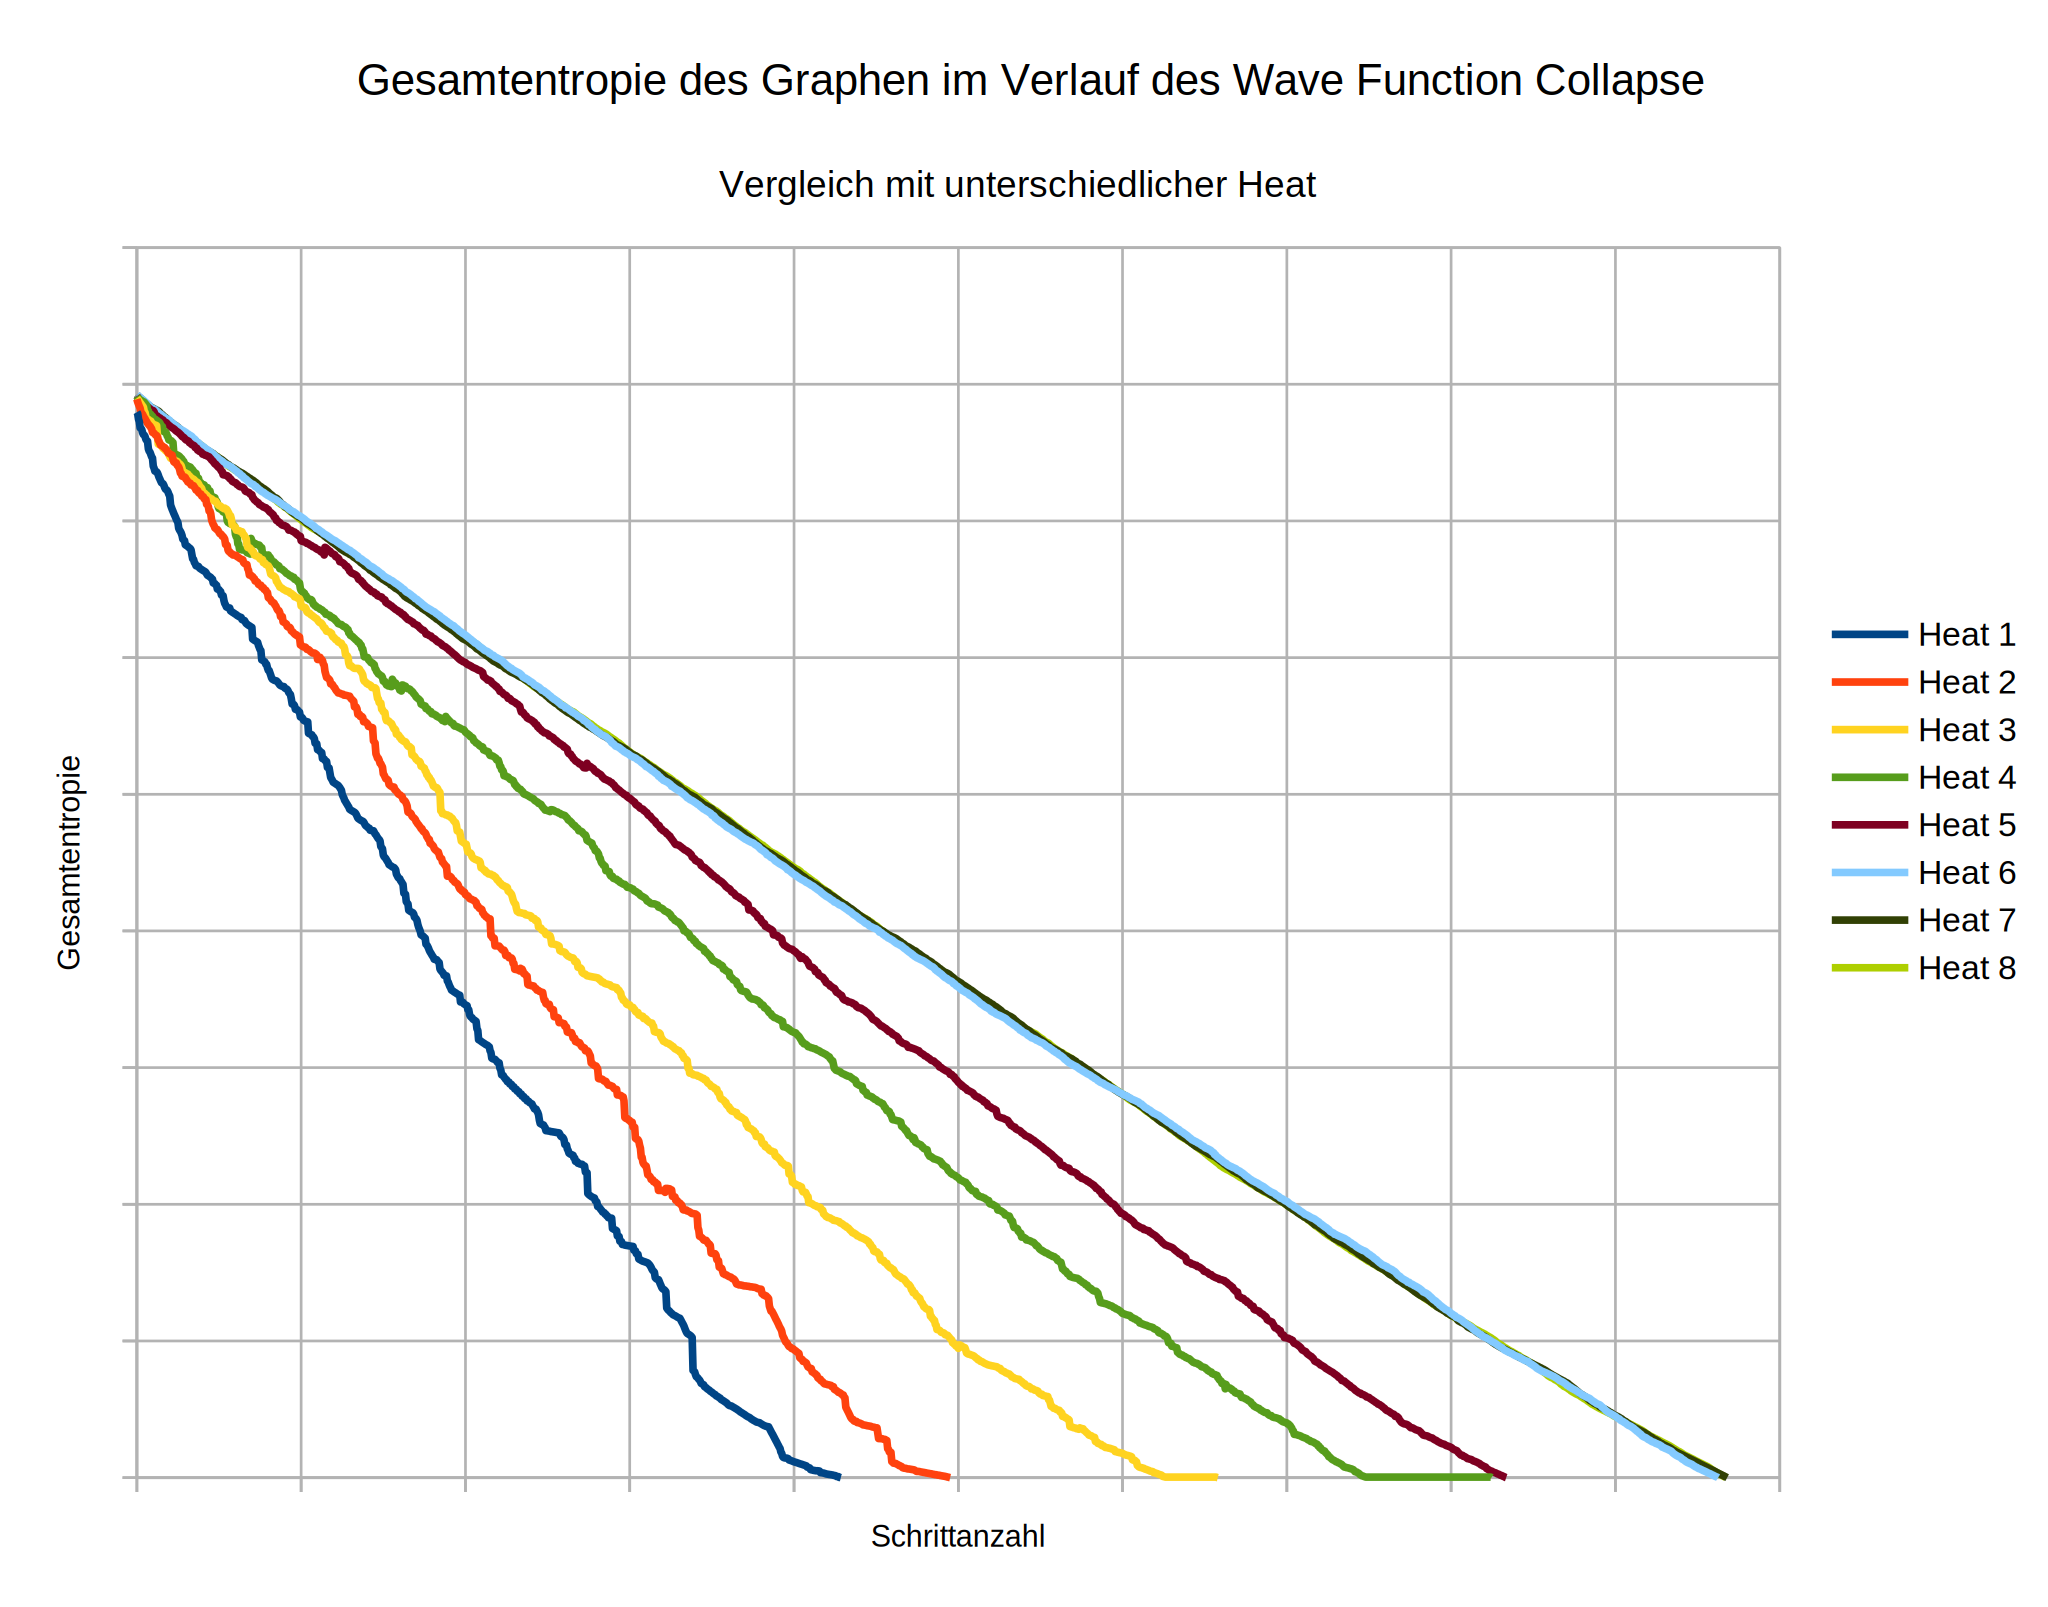
\includegraphics[width=\linewidth]{data/townscaper_grid/1.png} \caption{} \end{subfigure}
    \begin{subfigure}{0.18\textwidth} \includegraphics[width=\linewidth]{data/townscaper_grid/2.png} \caption{} \end{subfigure}
    \begin{subfigure}{0.18\textwidth} \includegraphics[width=\linewidth]{data/townscaper_grid/3.png} \caption{} \end{subfigure}
    \begin{subfigure}{0.18\textwidth} \includegraphics[width=\linewidth]{data/townscaper_grid/4.png} \caption{} \end{subfigure}
    \begin{subfigure}{0.18\textwidth} \includegraphics[width=\linewidth]{data/townscaper_grid/5.png} \caption{} \end{subfigure}
    
    \caption{
        Generierung eines Teils des Gitters für Townscaper \cite{stalberg_grid}. (a) Punkte werden generiert. (b) Triangulierung. (c) Kanten werden gelöscht, so dass Vierecke entstehen. (d) die Vierecke werden geviertelt. (e) Position der Knoten wird aufgelockert, so dass die Winkel zwischen Kanten gleichmäßiger sind.
    }
    \label{fig:townscaper_grid}
\end{figure}
\begin{figure}[H]
    \centering
    \begin{subfigure}{0.18\textwidth} 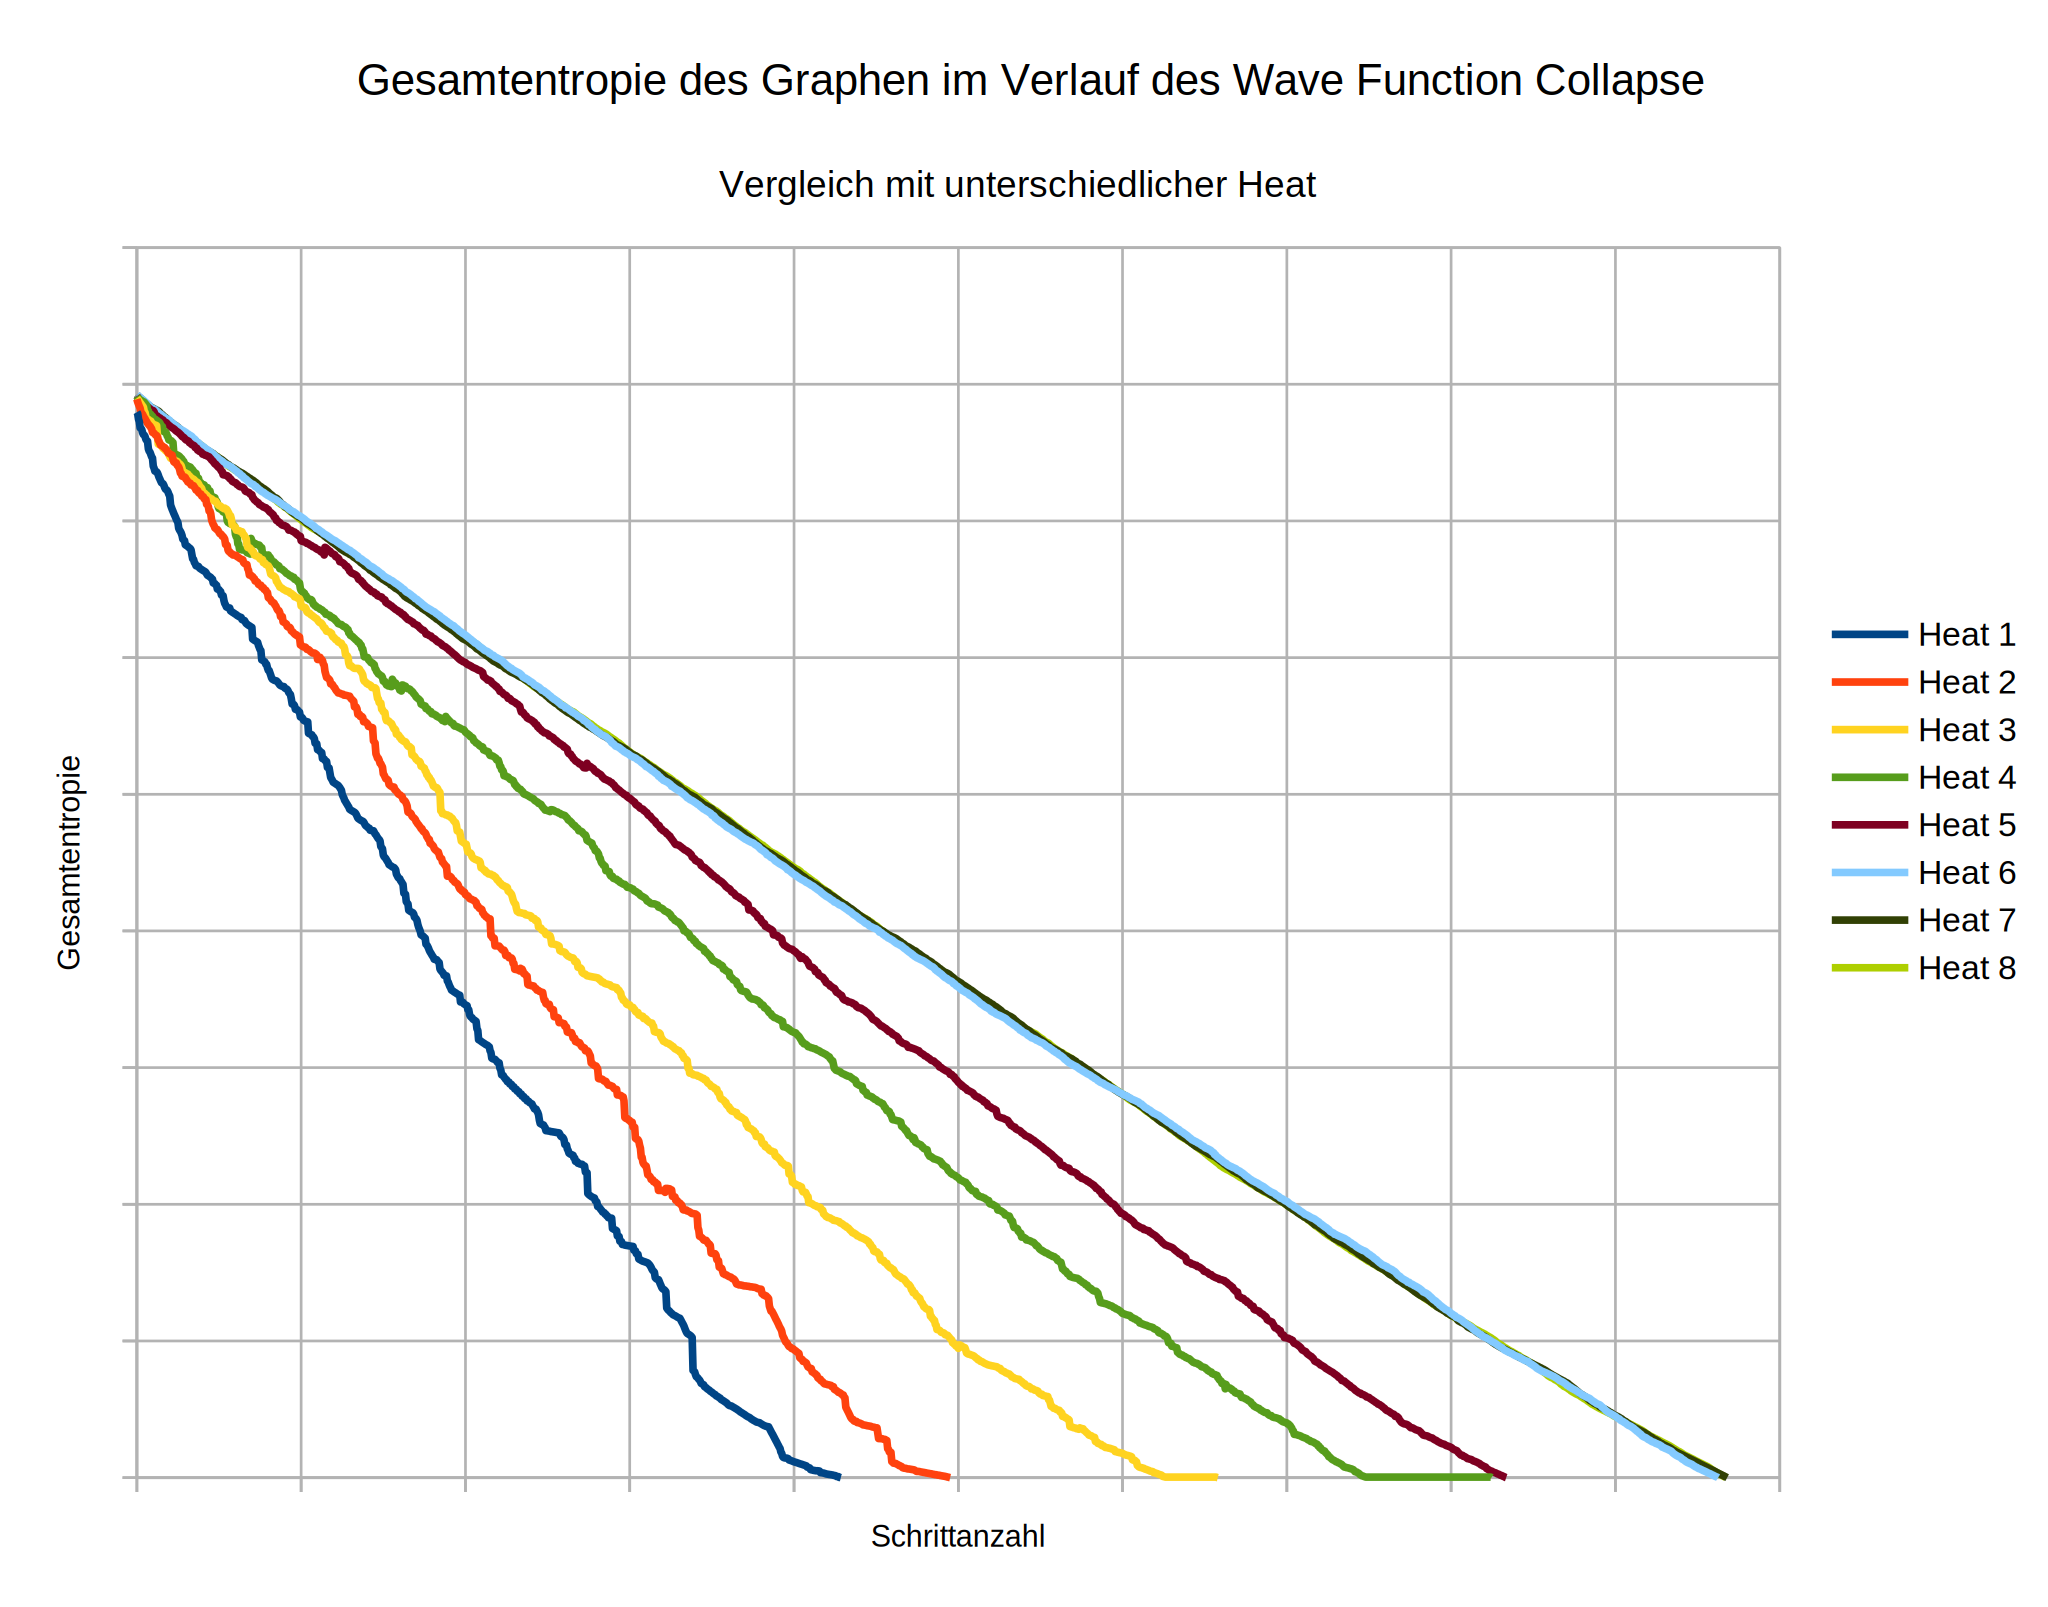
\includegraphics[width=\linewidth]{data/townscaper_grid/1.png} \caption{} \end{subfigure}
    \begin{subfigure}{0.18\textwidth} \includegraphics[width=\linewidth]{data/townscaper_grid/2.png} \caption{} \end{subfigure}
    \begin{subfigure}{0.18\textwidth} \includegraphics[width=\linewidth]{data/townscaper_grid/3.png} \caption{} \end{subfigure}
    \begin{subfigure}{0.18\textwidth} \includegraphics[width=\linewidth]{data/townscaper_grid/4.png} \caption{} \end{subfigure}
    \begin{subfigure}{0.18\textwidth} \includegraphics[width=\linewidth]{data/townscaper_grid/5.png} \caption{} \end{subfigure}
    
    \caption{
        Generierung eines Teils des Gitters für Townscaper \cite{stalberg_grid}. (a) Punkte werden generiert. (b) Triangulierung. (c) Kanten werden gelöscht, so dass Vierecke entstehen. (d) die Vierecke werden geviertelt. (e) Position der Knoten wird aufgelockert, so dass die Winkel zwischen Kanten gleichmäßiger sind.
    }
    \label{fig:townscaper_grid}
\end{figure}
\begin{figure}[H]
    \centering
    \begin{subfigure}{0.18\textwidth} 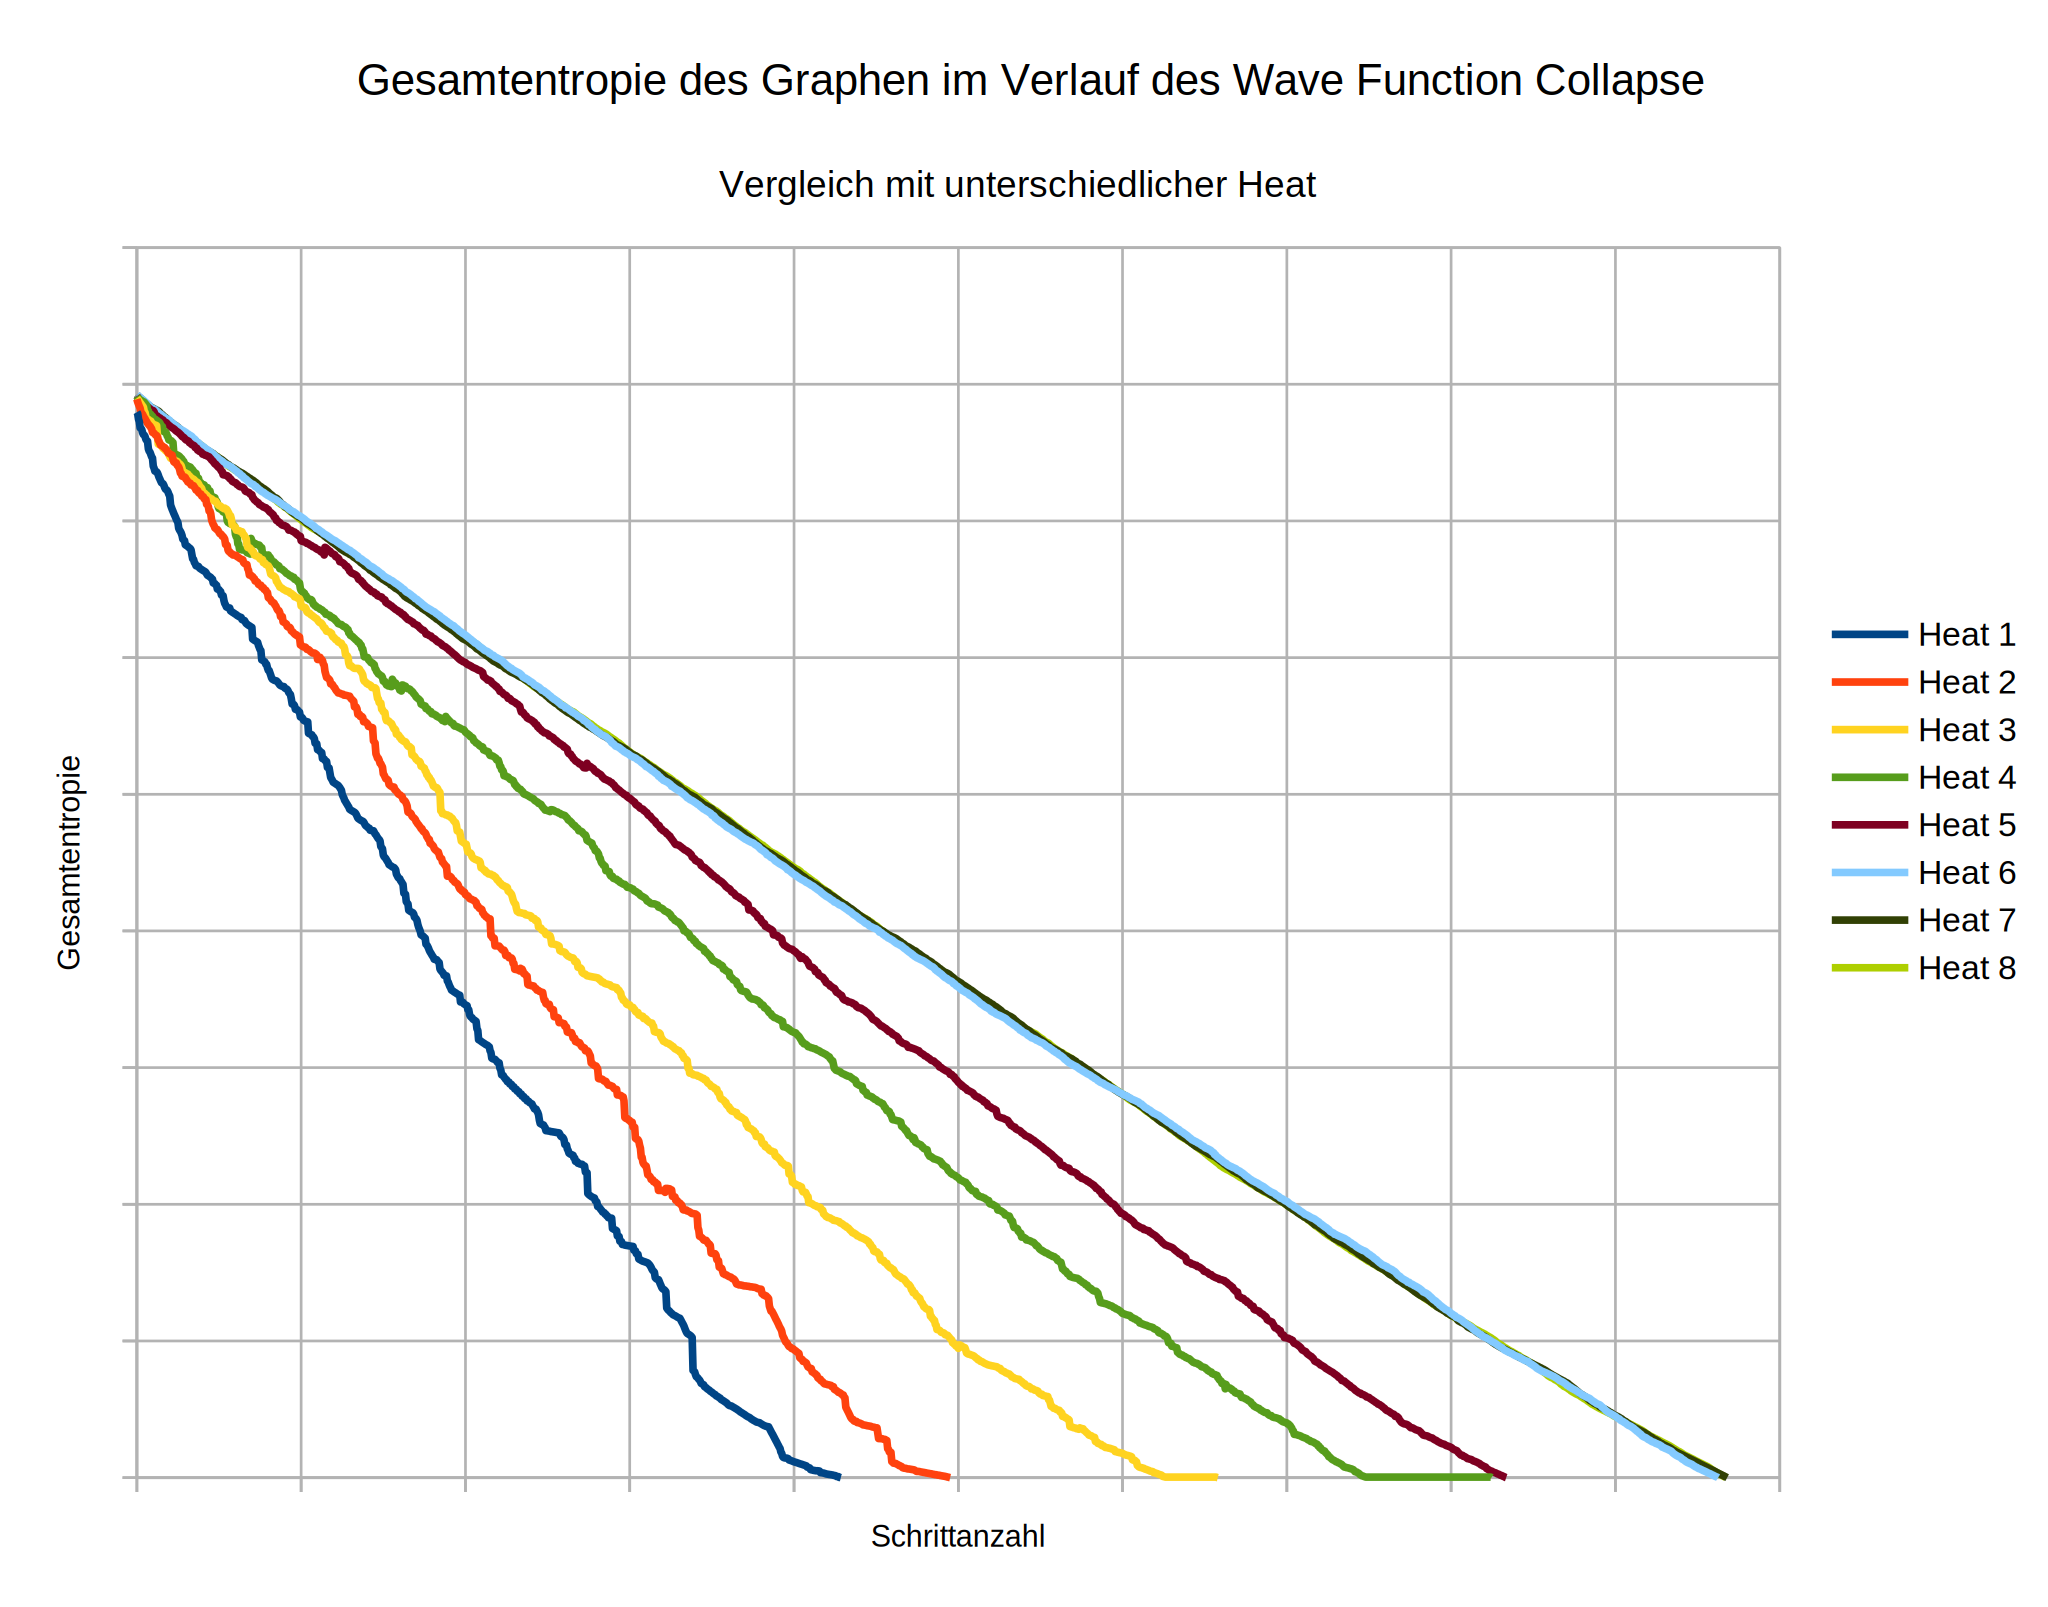
\includegraphics[width=\linewidth]{data/townscaper_grid/1.png} \caption{} \end{subfigure}
    \begin{subfigure}{0.18\textwidth} \includegraphics[width=\linewidth]{data/townscaper_grid/2.png} \caption{} \end{subfigure}
    \begin{subfigure}{0.18\textwidth} \includegraphics[width=\linewidth]{data/townscaper_grid/3.png} \caption{} \end{subfigure}
    \begin{subfigure}{0.18\textwidth} \includegraphics[width=\linewidth]{data/townscaper_grid/4.png} \caption{} \end{subfigure}
    \begin{subfigure}{0.18\textwidth} \includegraphics[width=\linewidth]{data/townscaper_grid/5.png} \caption{} \end{subfigure}
    
    \caption{
        Generierung eines Teils des Gitters für Townscaper \cite{stalberg_grid}. (a) Punkte werden generiert. (b) Triangulierung. (c) Kanten werden gelöscht, so dass Vierecke entstehen. (d) die Vierecke werden geviertelt. (e) Position der Knoten wird aufgelockert, so dass die Winkel zwischen Kanten gleichmäßiger sind.
    }
    \label{fig:townscaper_grid}
\end{figure}
\begin{figure}[H]
    \centering
    \begin{subfigure}{0.18\textwidth} 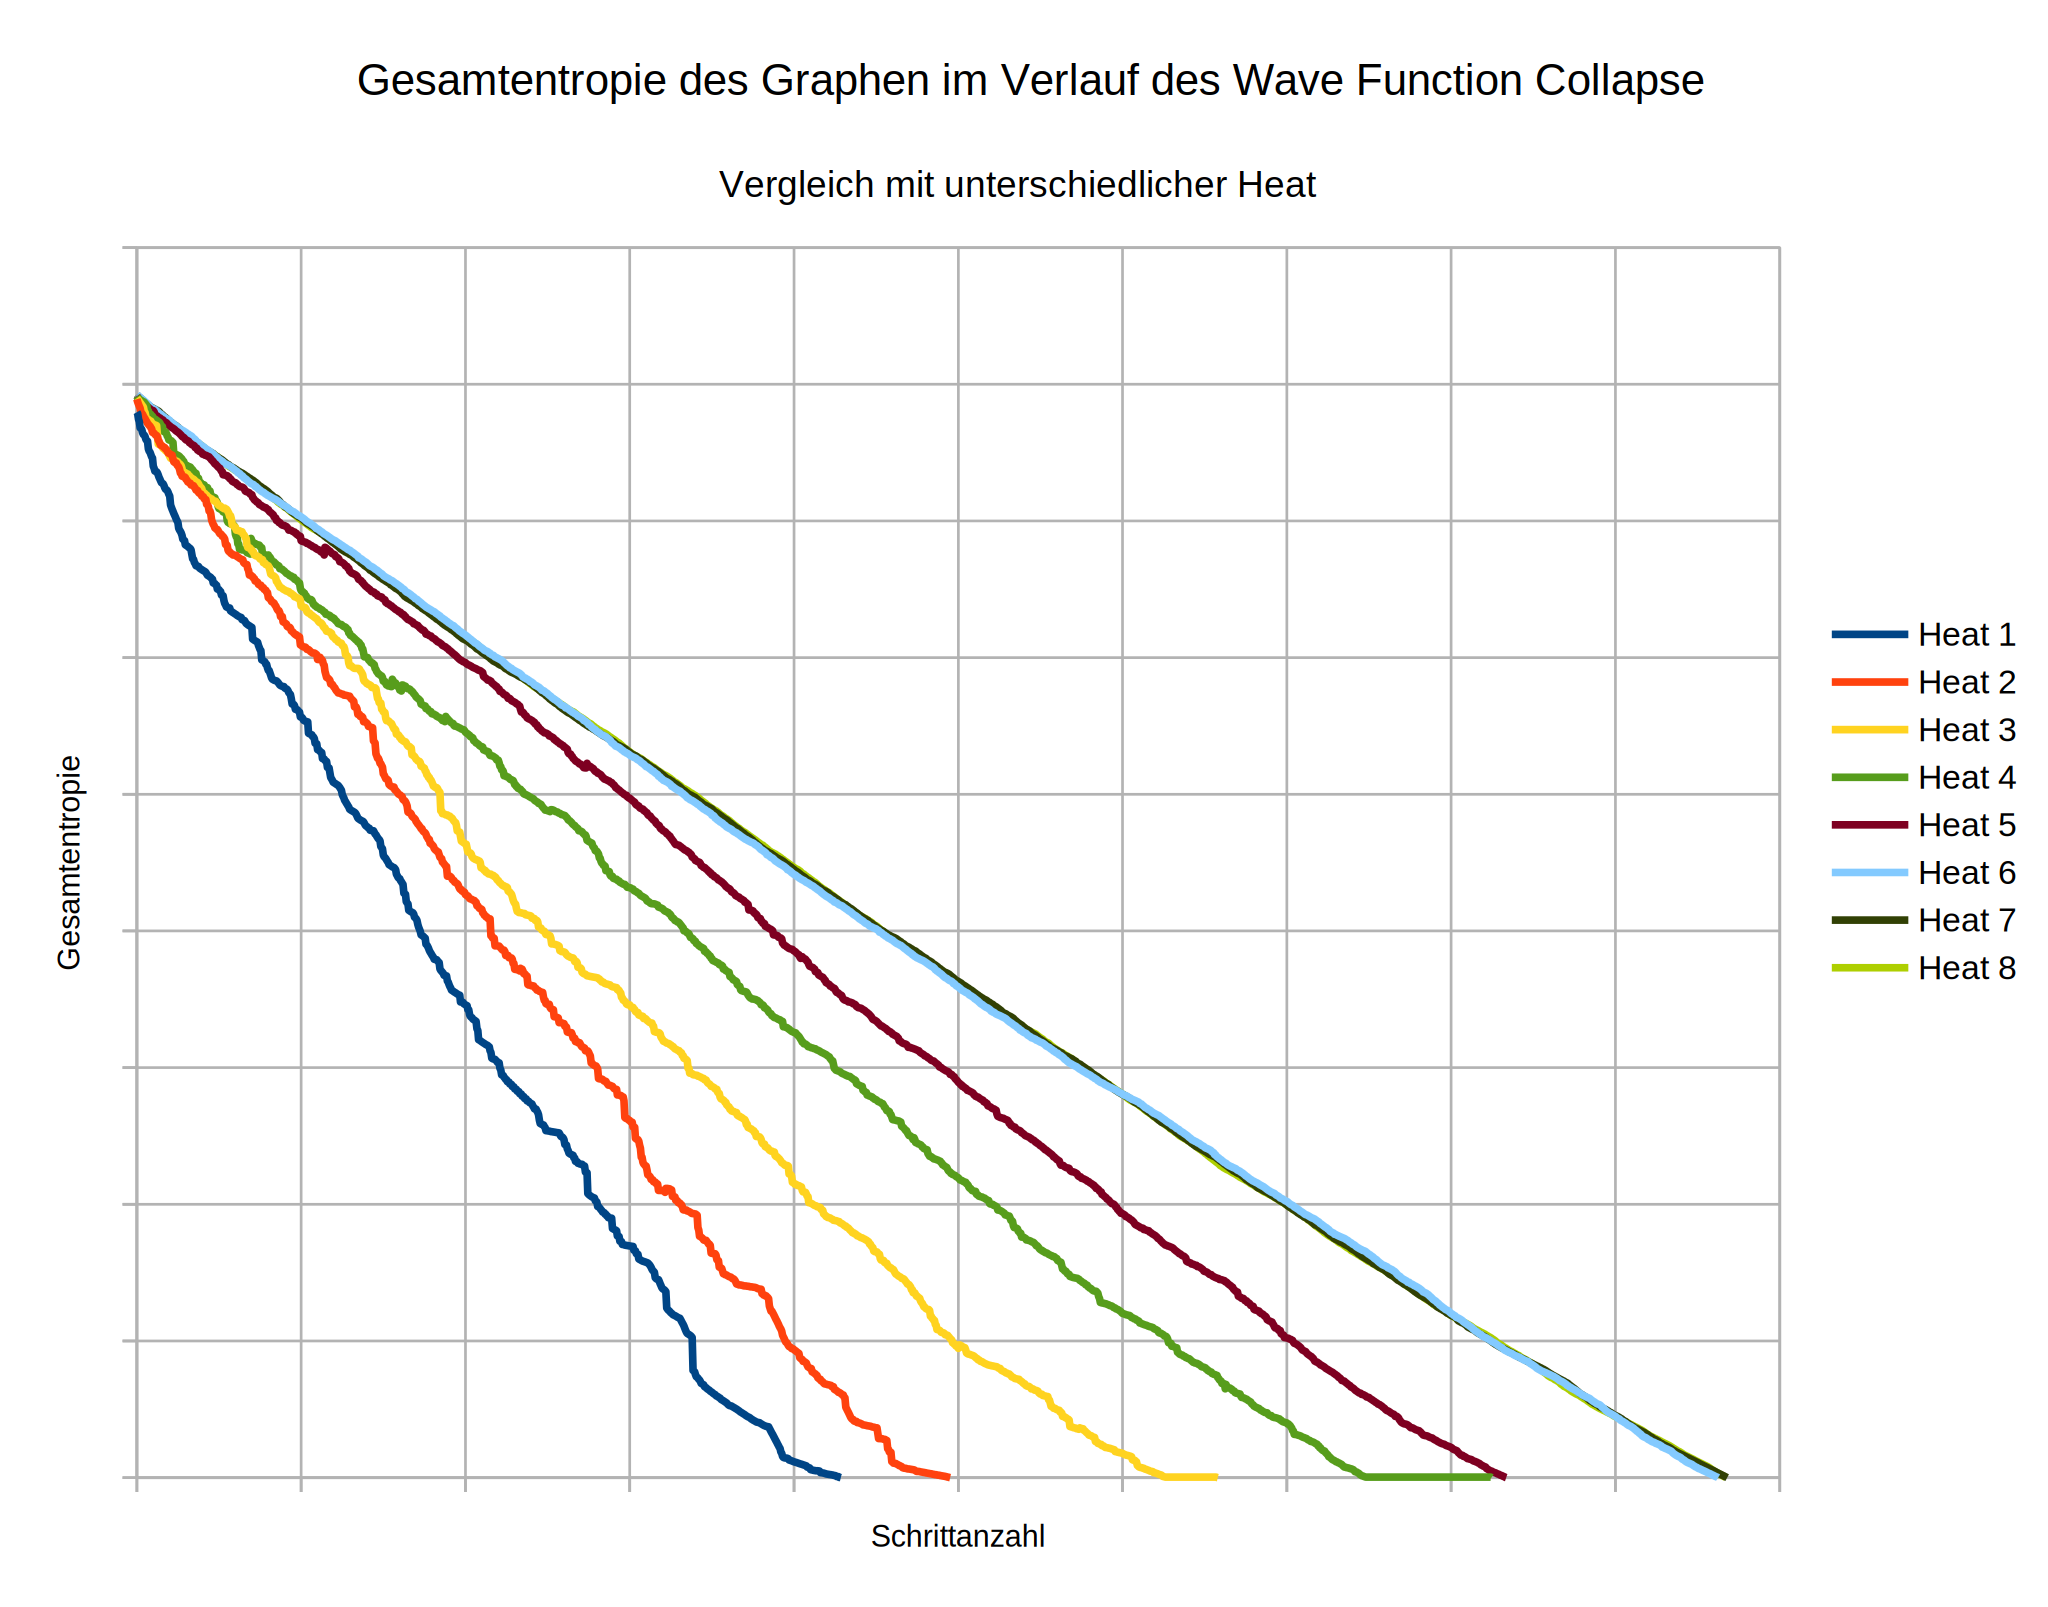
\includegraphics[width=\linewidth]{data/townscaper_grid/1.png} \caption{} \end{subfigure}
    \begin{subfigure}{0.18\textwidth} \includegraphics[width=\linewidth]{data/townscaper_grid/2.png} \caption{} \end{subfigure}
    \begin{subfigure}{0.18\textwidth} \includegraphics[width=\linewidth]{data/townscaper_grid/3.png} \caption{} \end{subfigure}
    \begin{subfigure}{0.18\textwidth} \includegraphics[width=\linewidth]{data/townscaper_grid/4.png} \caption{} \end{subfigure}
    \begin{subfigure}{0.18\textwidth} \includegraphics[width=\linewidth]{data/townscaper_grid/5.png} \caption{} \end{subfigure}
    
    \caption{
        Generierung eines Teils des Gitters für Townscaper \cite{stalberg_grid}. (a) Punkte werden generiert. (b) Triangulierung. (c) Kanten werden gelöscht, so dass Vierecke entstehen. (d) die Vierecke werden geviertelt. (e) Position der Knoten wird aufgelockert, so dass die Winkel zwischen Kanten gleichmäßiger sind.
    }
    \label{fig:townscaper_grid}
\end{figure}




\bibliographystyle{plain}
\bibliography{my}

\end{document}